\documentclass[letter]{article}
\usepackage[margin=1in]{geometry}
\usepackage{amsmath, amssymb}
\usepackage{enumerate}
\usepackage{graphicx}
\usepackage{fancyhdr}

\pagestyle{fancy}
\fancyhead[L]{STAT 542 HW6}
\fancyhead[R]{Xin Yin}

\newcommand{\sqtpi}{\sqrt{2\pi}}
\newcommand{\Gal}{\Gamma(\alpha)}
\newcommand{\Iy}{\frac{1}{y}}
\newcommand{\Beal}{\beta^\alpha}
\newcommand{\intzi}{\int_0^\infty}

\begin{document}
    \section*{3.11}
    \begin{enumerate}[(a)]
    \item 
    \begin{align*}
    P(X=x|N,M,K) & = \frac{\binom{M}{x} \binom{N-M}{K-x}}{\binom{N}{k}} 
    = \frac{\frac{M!}{(M-x)!x!} \frac{(N-M)!}{(N-M-K+x)!(K-x)!}}{\frac{N!}{(N-K)!K!}} \\
    & = \frac{K!}{(K-x)!x!} \frac{M(M-1)\cdots(M-x+1) \cdot (N-M) \cdots (N-M-K+x+1)}{N(N-1)\cdots(N-K+1)}\\
    & \text{Note that in the second ratio, both parts have $K = x + (K-x)$ terms}\\
    & = \binom{K}{x} \left(\frac{M}{N} \frac{M}{N-1} \cdots \frac{M-x+1}{N-x+1} \right) \left(\frac{N-M}{N-x} \frac{N-M-1}{N-x-1} \frac{N-M-K-x+1}{N-k+1} \right)
    \end{align*}
    Therefore
    \[
    \lim_{N \to \infty, M \to \infty, M/N \to p} P(X=x|N,M,K) = \binom{K}{x} \left(\frac{M}{N}\right)^x \left(\frac{N-M}{N}\right)^{K-x} = \binom{K}{x} p^x (1-p)^{K-x}
    \]

    \item Since Poisson$(\lambda)$ can be used as approxmiation of binomial$(n, p)$, as $n \to \infty, p \to 1$, where $\lambda = np$. Using the results from (a), as $N\to\infty, M\to\infty, M/N\to p$, 
    the hypergeometric can be approxmiated by binomial$(K, M/N)$.

    Now, given that $K\to\infty, N/M\to 0, KM/N\to\lambda$, it satisfies the condition for Poisson approximation, and $\lambda = KM/N$. Therefore, 
    \[
    P(X=x|N,M,K) \to \frac{e^{-\lambda}\lambda^x}{x!}, x = 0, 1, \dots
    \]
    as $N\to\infty, M\to\infty, M/N\to 0, KM/N\to\lambda$.
    \item
    \begin{flalign*}
    & P(X=x|N,M,K) = \frac{\binom{M}{x} \binom{N-M}{K-x}}{\binom{N}{k}} =
    \frac{\frac{M!K!}{(M-x)!(K-x)!}}{x!} \frac{(N-M)!(N-K)!}{(N-M-K+x)!N!} \\
     & = \frac{\frac{M(M-1)\cdots(M-X+1)K(K-1)\cdots(K-x+1)}{N(N-1)\cdots(N-x+1)}}{x!} \frac{(N-M)!(N-K)!}{(N-x)!(N-M-K+x)!}\\
    \\
    & \lim_{N\to\infty, M\to\infty, K\to\infty, N/M\to 0, KM/N\to \lambda}
    \frac{\frac{M(M-1)\cdots(M-X+1)K(K-1)\cdots(K-x+1)}{N(N-1)\cdots(N-x+1)}}{x!} = 
    \frac{\left(\frac{KM}{N}\right)^x}{x!} = \frac{\lambda^x}{x!} \\
     \\
    & \lim_{N\to\infty, M\to\infty, K\to\infty, N/M\to 0, KM/N\to \lambda} 
    \frac{(N-M)!(N-K)!}{(N-x)!(N-M-K+x)!} = \\
    &  = \lim \frac{(N-M)(N-1-M)\cdots(N-K+1-M)(N-K)!}{(N-x)(N-1-x)\cdots(N-K+1)(N-K)!} \\
    & = \lim \left(\frac{N}{N-x}-\frac{MK}{(N-x)K}\right)\left(\frac{N-1}{N-1-x}-\frac{MK}{K(N-1-x)}\right)\cdots\left(\frac{N-K+x+1}{N-K+1}-\frac{MK}{K(N-K+1)}\right) \\
    & = \lim \left(1-\frac{\frac{MK}{N}}{K}\right)^{K-x} = \left(1-\frac{\lambda}{K}\right)^K = e^{-\lambda}\\
    \end{flalign*}
    \end{enumerate}
    Hence, as $N\to\infty, M\to\infty, K\to\infty, N/M \to 0, KM/N \to \lambda$, 
    \[
    P(X=x|N,M,K) = \frac{e^{-\lambda} \lambda^x}{x!}
    \]

    \section*{3.12}
    Since X has $\text{binomial}(n,p)$, we know that,
    \[
    F_X(r-1) = P_X(X \le r-1) = P_X(\text{$r-1$ successes within $n$ Bernoulli trials}) \\
    \]
    Namely, we have $n-(r-1) = n-r+1$ failures in $n$ trials. It is obvious that we will have at least $n-r+1$ failures before the $r$-th success.
    So,
    \[
    F_X(r-1) = P(\text{at least $n-r+1$ failures before $r$ successes})
    \]
    We notice that this will, by definition, follow a negative binomial$(r, p)$. If we use $Y$ to denote the number of failures, we can write down the above probability as,
    \[
    F_X(r-1) = P_Y(Y \ge n-r+1) = 1 - P_Y(Y \le n-r)  = 1- F_Y(n-r).
    \]
    \section*{3.13}
    \begin{enumerate}[(a)]
    \item If $X \sim \text{Poisson}(\lambda)$, 
    \[
    P(X > 0) = 1 - P(X = 0) = 1 - \frac{e^{-\lambda} \lambda^0}{0!} = 1 - e^{-\lambda}
    \]
    So, the truncated Poisson is,
    \[
    P(X_T = x) = \frac{P(X=x)}{P(X > 0)} = \frac{\frac{e^{-\lambda} \lambda^x}{x!}}{1-e^{-\lambda}}, x = 1, 2, \dots
    \]
    \item $X \sim \text{negative binomial}(r, p)$,
    \[
    P(X = 0) = \binom{-r}{0} p^r(p-1)^0 = p^r
    \]
    So,
    \[
    P(X_T = x) = \frac{P(X=x)}{P(X > 0)} = \frac{\binom{-r}{x} p^r (p-1)^x}{1-p^r}
    \]
    \end{enumerate}

    \section*{3.19}
    \begin{align*}
    \int_x^\infty \frac{1}{\Gamma(\alpha)} z^{\alpha-1} e^{-z} dz & =
    \frac{-1}{\Gamma(\alpha)} \int_x^\infty z^{\alpha-1} d e^{-z} \\
    & = \left. \frac{1}{\Gamma(\alpha)} z^{\alpha-1}e^{-z} \right|^x_\infty + 
    \int_x^\infty \frac{\alpha-1}{\Gamma(\alpha)} z^{\alpha-2}e^{-z} dz\\
    & \text{Using L'Hopital's rule, we have, $\lim_{x\to \infty} z^{\alpha-1} e^{-z} = 0$},\\
    & \text{also we have $\frac{\alpha-1}{\Gamma(\alpha)} = \frac{1}{\Gamma(\alpha-1)}$}, \\
    & = \frac{x^{\alpha-1}e^{-x}}{(\alpha-1)!} + \int_x^\infty \frac{1}{\Gamma(\alpha-1)} z^{\alpha-2} e^{-z}dz.
    \end{align*}
    So, we have recursive relationship,
    \[
    \int_x^\infty gamma(\alpha, 1) = \frac{x^{\alpha-1}e^{-x}}{(\alpha-1)!}  + \int_a^\infty gamma(\alpha-1, 1)
    \]
    To expand this recursive relationship, it can be easily seen that,
    \[
    \int_x^\infty \frac{1}{\Gamma(\alpha)} z^{\alpha-1} z^{-x} dx = \frac{x^{\alpha-1}e^{-x}}{(\alpha-1)!} + \frac{x^{\alpha-2}e^{-x}}{(\alpha-2)!} + \dots + \frac{x^{0}e^{-x}}{0!}
    \]
    \emph{i.e.}
    \[
    \int_x^\infty \frac{1}{\Gamma(\alpha)} z^{\alpha-1} e^{-z} dz = \sum_{y=0}{\alpha-1} \frac{x^y e^{-x}}{y!}
    \]
    And this implies that, if $X \sim gamma(\alpha, 1)$, we will have,
    \[
    P_X(X \ge x) = P_Y(Y \le \alpha-1),
    \]
    where $Y \sim \text{Poisson}(x)$.
    \section*{3.20}
    Since X has pdf,
    \[
    f(x) = \frac{2}{\sqtpi} e^{-x^2/2}, 0 < x < \infty
    \]
    \begin{enumerate}[(a)]
        \item 
        \begin{align*}
        EX & = \intzi \frac{2}{\sqtpi} x e^{-x^2/2} dx = -\intzi \frac{2}{\sqtpi} d e^{-x^2/2}
        = \left. \frac{2}{\sqtpi} e^{-x^2/2} \right|^0_\infty = \frac{2}{\sqtpi} \\
        EX^2 & = \intzi \frac{2}{\sqtpi} x^2 e^{-x^2/2} dx \\
        & \text{Use integration by parts}, \\
        & = \left. \frac{2}{\sqtpi} x e^{-x^2/2} \right|_\infty^0 + \intzi \frac{2}{\sqtpi} x e^{-x^2/2} dx = \frac{2}{\sqtpi}\\
        Var(X) & = EX^2 - (EX)^2 = \frac{\sqtpi -2}{\pi}
        \end{align*}
        \item $\Gamma(1/2) = \sqrt{\pi}$. Given transformation $Y = g(X)$, we can write down $f_Y(y)$ as,
        \[
        f_Y(y)  = f_X(g^{-1}(y)) \left| \frac{d g^{-1}(y)}{dy} \right|
        = \frac{2}{\sqrt{2} \Gamma(1/2)} e^{-\frac{g^{-1}(y)^2}{2}} \left| \frac{d g^{-1}(y)}{dy} \right|
        \]
        Notice that to match the pdf of a \emph{Gamma} distribution, $g^{-1}(y)$ should have the form $c\sqrt{y}$, where $c$ is a non-zero constant. Therefore 
        $\frac{d}{dy} g^{-1}(y) = \frac{2}{c} y^{-1/2} = \frac{2}{c} y^{1/2-1}$.
        Now, we can rewrite $f_Y(y)$ as,
        \[
        f_Y(y) = \frac{c}{\Gamma(1/2) 2^{1/2}} y^{1/2-1} e^{-c^2y/2}
        \]
        Apparently, $\alpha = 1/2, \beta = 2$, and to make this function a valid pdf or valid \emph{Gamma} density, we can find that $c=1$, so, $g^{-1}(y) = \sqrt{y}, Y=g(X)=X^2$.
    \end{enumerate}
    \section*{3.23}
    \begin{enumerate}[(a)]
        \item Because $\alpha > 0, \beta > 0, \alpha < x < \infty$, $f(x) > 0$.
        To show that integrate $f(x)$ over its support equals 1, 
        \[
        \int_\alpha^\infty \frac{\beta \alpha^\beta}{x^{\beta+1}} dx = \beta \alpha^\beta \int_\alpha^infty x^{-(\beta+1)} dx = \left. x^{-\beta} \alpha^\beta \right|^\alpha_\infty = 1.
        \]
        \item
        \[
        EX = \int_\alpha^\infty \frac{x \beta \alpha^\beta}{x^{\beta+1}} = 
        \beta \alpha^\beta \int_\alpha^\infty x^{-\beta} dx = \left. \frac{x^{-\beta+1}}{-\beta+1} \beta \alpha^\beta \right|^\infty_\alpha = \frac{\beta}{\alpha(\beta-1)}
        \]
        Notice that when $\beta < 1$, $EX < 0$ is impossible because $X > \alpha > 0$. So, $EX$ only exists when $\beta > 1$.
        \item 
        \begin{align*}
        EX^2 & = \int_\alpha^\infty \frac{\beta \alpha^\beta}{x^{\beta-1}} dx =
        \left. \frac{x^{-\beta+2}}{-\beta+2} \beta \alpha^\beta \right|_\alpha^\infty = \frac{\beta}{(\beta-2)\alpha^2} \\
        Var(X) &= EX^2 - (EX)^2 = \frac{\beta}{(\beta-2)\alpha^2} - \frac{\beta^2}{\alpha^2 (\beta-1)^2} = \frac{\beta}{\alpha^2 (\beta-1)^2 (\beta-2)}
        \end{align*}
        So, when $\beta < 2$, $Var(X) < 0$ is invalid. Or, $\beta = 2, Var(X) = \infty$. Thus, $Var(X)$ doesn't exist if $\beta \le 2$.
    \end{enumerate}

    \section*{3.24}
    \begin{enumerate}[(a)]
    \item Given that $f_X(x) = \frac{1}{\beta} e^{-x/\beta}, 0 < x <\infty$ and $Y = X^{1/\gamma}, 0 < x < \infty$, we know that, $g^{-1}(y) = y^\gamma$.
    Therefore,
    \[
    f_Y(y) = \frac{1}{\beta} e^{-y^\gamma/\beta} \left| \frac{d}{dy} y^\gamma \right| = \frac{\gamma}{\beta} e^{-y^\gamma/\beta} y^{\gamma-1}
    \]

    It can be easily shown that,
    \[
    \intzi \frac{\gamma}{\beta} e^{-y^\gamma/\beta} y^{\gamma-1} dy = \left. e^{-y^\gamma/\beta} \right|^0_\infty = 1.
    \]
    Also, $f_Y(y)$ is nonnegative, given $y > 0, \gamma > 0$. So, $f_Y(y)$ is a pdf.

    Using integration by parts, we can show that,
    \begin{align*}
    EY & = \intzi y \frac{\gamma}{\beta} e^{-y^\gamma/\beta} y^{\gamma-1} dy = \left. y e^{-y^\gamma/\beta} \right|^0_\infty + \intzi e^{-y^\gamma/\beta} y^{\gamma-1} dy \\
    & \text{Because $x = y^\gamma, y = x^{1/\gamma}$},\\
    & = \intzi e^{-x/\beta} dx^{1/\gamma} = \intzi \frac{1}{\gamma} e^{-x/\beta} x^{1/\gamma -1} dx \\
    & \text{Let $\alpha = 1/\gamma$},\\
    & = \intzi \alpha e^{-x/\beta}  x^{\alpha-1} dx = \alpha \Gamma(\alpha) \beta^\alpha \intzi \frac{1}{\Gamma(\alpha)\beta^\alpha} e^{-x/\beta} x^{\alpha-1}dx \\
    & \text{Notice that the integral is a gamma density, we have},\\
    & = \Gamma(1 + 1/\gamma) \beta^{1/\gamma}\\
    & \text{Similarly},\\
    EY^2 & = \left. y^2 e^{-y^\gamma/\beta} \right|^0_\infty + \intzi 2e^{-y^\gamma/\beta} y dy \\
    & = 2 \intzi e^{-x/\beta} \frac{1/\gamma} x^{1/\gamma} x^{1/\gamma-1} dx = \intzi \frac{2}{\gamma} e^{-x/\beta} x^{2/\gamma -1} dx \\
    & \text{Let $\alpha= 2/\gamma$},\\
    & = 2\Gamma(\alpha) \beta^\alpha \intzi \frac{1}{\Gamma(\alpha)\beta^\alpha} e^{-x/\beta} x^{\alpha-1} dx \\
    & = \Gamma(1+2/\gamma) \beta^{2/\gamma}\\
    \\
    Var(Y) & = EY^2 - (EY)^2 = \beta^{2/\gamma}\left[\Gamma(1+2/\gamma) - \Gamma^2(1+1/\gamma)\right]
    \end{align*}
    \item $f_X(x) = \frac{1}{\beta} e^{-x/\beta}, 0 < x < \infty$, $Y=\sqrt{2X/\beta}, 0 < y < \infty$, $g^{-1}(y) = \beta y^2/2$. 
    \[
    f_Y(y) = \frac{1}{\beta} e^{-y^2/2}\beta y = y e^{-y^2/2}, 0 < y < \infty.
    \]
    which is nonnegative, as $y > 0$.
    \[
    \intzi ye^{-y^2/2} = \left. e^{-y^2/2} \right|^0_\infty = 0.
    \]
    So $f_Y$ is a valid pdf.
    \begin{align*}
    EY & = \intzi y^2 e^{-y^2/2}dy = \left.y e^{-y^2/2}\right|^0_\infty + \intzi e^{-y^2/2}dy \\
    & = \sqtpi \intzi \frac{1}{\sqtpi} e^{-y^2/2}dy = \sqrt{\pi/2} \int_{-infty}^\infty \frac{1}{\sqtpi} e^{-y^2/2}dy \\
    & \text{The integrand is the standard normal density, so},\\
    & = \sqrt{\frac{\pi}{2}}.\\
    \\
    EY^2 & = \intzi y^3 e^{-y^2/2} dy = \left. y^2 e^{-y^2/2} \right|^0_infty + 2 \intzi ye^{-y^2/2} dy = 2.\\
    \\
    Var(Y) & = EY^2 - (EY)^2 = 2-\frac{pi}{2}
    \end{align*}
    \item 
    \begin{align*}
    f_X(x) & = \frac{1}{\Gal \Beal} x^{\alpha-1} e^{-x/\beta}, 0 < x < \infty \\
    Y & = 1/X, 0 < y < \infty, \quad g^{-1}(y) = 1/y.\\
    f_Y(y) & = \frac{1}{\Gal \Beal} (\frac{1}{y})^{\alpha-1} e^{-\frac{1}{y\beta}} \frac{1}{y^2} = 
    \frac{1}{\Gal \Beal} (\frac{1}{y})^{\alpha+1} e^{-\frac{1}{y\beta}} \\
    & \text{It can be easily shown that to integrate this pdf is equivalent to integrate a gamma density},\\
    & \text{by letting $u = 1/y$. Hence $f_Y$ is a pdf}.\\ 
    EY & = \intzi \frac{1}{\Gal \Beal} (\Iy)^\alpha e^{-1/\beta y} dy = \frac{\Gamma(\alpha-1)}{\Gal \beta} \intzi IG(\alpha-1, \beta) dy \\
    & = \frac{1}{(\alpha-1)\beta} \\
    & \text{Because $y > 0$, $EY$ only exists when $\alpha > 1$.}\\
    EY^2 & = \intzi \frac{1}{\Gal \Beal} (\Iy)^{\alpha-1} e^{-1/\beta y} dy = \frac{\Gamma(\alpha-2)}{\Gal \beta^2} \intzi IG(\alpha-2, \beta) dy \\
    & = \frac{1}{(\alpha-1)(\alpha-2)\beta^2}\\
    \\
    Var(Y) & = EY^2 - (EY)^2 = \frac{1}{(\alpha-1)^2(\alpha-2)\beta^2}, \alpha > 2
    \end{align*}
    \item
    \begin{align*}
    f_X(x) & = \frac{1}{\Gamma{3/2}\beta^{3/2}} x^{3/2-1} e^{-2x/3} = \frac{1}{\sqrt{\pi}/2 \beta^{3/2}} x^{1/2} e^{-2x/3}, 0 < x < \infty.\\
    Y & = \sqrt{X/\beta}, 0 < y < \infty, g^{-1}(y) = \beta y^2 \\
    f_Y(y) & = \frac{1}{\sqrt{\pi}/2 \beta^{3/2}} (\beta y^2)^{1/2} e^{-y^2} 2\beta y = \frac{4}{\sqrt{\pi}} y^2 e^{-y^2}\\
    \end{align*}
    Let $u = y/\sqrt{2}$,
    \[
    \intzi \frac{4}{\sqrt{\pi}} y^2 e^{-y^2}  = \frac{4}{\sqrt{\pi}} \intzi \frac{u^2}{2\sqrt{2}} e^{-u^2/2}du
    \]
    Notice the integral is what we've computed in (b), which equals to $\sqrt{\pi/2}$. 
    
    Then,
    \[
    \intzi \frac{4}{\sqrt{\pi}} y^2 e^{-y^2} = \sqrt{\frac{2}{\pi}} \sqrt{\frac{\pi}{2}} = 1.
    \]

    \begin{align*}
    EY & = \intzi \frac{4}{\sqrt{\pi}} y^3 e^{-y^2} dy = \left. \frac{2}{\sqrt{\pi}} y^2 e^{-y^2} \right|^0_\infty + \intzi \frac{4}{\sqrt{\pi}} y e^{-y^2} dy \\
    & = 0 + \left. \frac{2}{\sqrt{\pi}} e^{-y^2} \right|^0_\infty = \frac{2}{\sqrt{\pi}} \\
    EY^2 & = \frac{4}{\sqrt{\pi}} y^3 e^{-y^2} dy = \frac{2}{\sqrt{\pi}} y^3 e^{-y^2} + \intzi \frac{6}{\sqrt{\pi}} y^2 e^{-y^2}dy = 3/2\\
    \\
    Var(Y) &= EY^2 - (EY)^2 = \frac{3}{2} - \frac{4}{\pi}
    \end{align*}

    \item 
    \begin{align*}
    f_X(x) & = e^{-x}, 0 < x < \infty.\\
    Y & = \alpha - \gamma\log X, -\infty < y < \infty, \quad g^{-1}(y) = e^{\frac{\alpha-y}{\gamma}}\\
    f_Y(y) &= e^{-e^{\frac{\alpha-y}{\gamma}}} \frac{1}{\gamma} e^{\frac{\alpha-y}{\gamma}}\\
    \end{align*}
    It can be easily shown that this density integrates to 1 on $(-\infty, infty)$. Given that $e^(\cdot)$ is nonnegative, $f_Y$ is a pdf.
    \begin{align*}
    EY & = \intzi (\alpha - \gamma \log x) e^{-y} dy = \alpha - \gamma \intzi \log y e^{-y} dy\\
    EY^2 & = \intzi (\alpha - \gamma \log x)^2 e^{-y} dy = \alpha^2 -\alpha \gamma \intzi \log y e^{-y} dy + \gamma^2 \intzi \log^2 y e^{-y} dy \\
    \end{align*}
    The integral $-\intzi \log x e^{-x} dx$ is equal to Euler-Mascheroni constant, which will be denoted $\epsilon$ below for convenience. Also, $\intzi \log^2 y e^{-y} dy = \epsilon^2 + \frac{1}{6} \pi^2.$
    Therefore,
    \begin{align*}
    EY & = \alpha + \gamma \epsilon \\
    EY^2 & = \alpha^2 + 2\alpha\gamma\epsilon + \gamma^2 (\epsilon^2 + \frac{1}{6} \pi^2)\\
    Var(Y) & = EY^2 - (EY)^2 = \frac{1}{6} \pi^2 \gamma^2
    \end{align*}
    \end{enumerate}

    \section*{3.26}
    \begin{enumerate}[(a)]
    \item Given that $T \sim exp(\beta)$, $F_T(t) = 1 - e^{-t/\beta}$, 
    \[
    h_T(t) = -\frac{d}{dt}\log(1-(1-e^{-t/\beta})) = -\frac{d}{dt}\frac{-t}{\beta} = 1/\beta
    \]
    \item If $T \sim \text{Weibull}(\gamma, \beta)$, we know that, from Exercise $3.24$, 
    \[
    f_T(t) = \frac{\gamma}{\beta} e^{-y^\gamma/\beta} y^{\gamma-1}
    \]
    So,
    \[
    F_T(t) = \int_0^t \frac{\gamma}{\beta} e^{-t^\gamma/\beta} t^{\gamma -1} dt = 1-e^{-t^\gamma/\beta}
    \]
    and,
    \[
    h_T(t) = \frac{f_T(t)}{1-F_T(t)} = \frac{\frac{\gamma}{\beta} e^{-t^\gamma/\beta} t^{\gamma-1}}{e^{-t^\gamma/\beta}} = \frac{\gamma t^{\gamma-1}}{\beta}
    \]
    \item Given the cdf of a logistic distribution, $F_T(t) = \frac{1}{1+e^{-(t-\mu)/\beta}}$, we can compute the hazard function as,
    \begin{align*}
    h_T(t) & = -\frac{d}{dt} \log(1-F_T(t)) = -\frac{d}{dt} \log(e^{-(t-\mu)/\beta}) - \log(1+e^{-(t-\mu)/\beta}) \\
    & = \frac{1}{\beta} - \frac{e^{-(t-\mu)\beta}}{\beta(1+e^{-(t-\mu)/\beta})} = \frac{1}{\beta(1+e^{-(t-\mu)/\beta})} = \frac{1}{\beta} F_T(t).
    \end{align*}
    \end{enumerate}

    \section*{3.44}
    Given that $g(X) = |X|$ is a nonnegative function, we can easily get, using Chebychev's Inequality, that,
    \[
    P(|X| \ge b) \le \frac{E|X|}{b}.
    \]
    Also, using the property of inequality, we know that $P(|X| \ge b) = P(X^2 \ge b^2)$. We could apply Chebychev's Inequality again, given $g(X) = X^2$ is nonnegative,
    \[
    P(|X| \ge b) = P(X^2 \ge r^2) \le \frac{EX^2}{b^2}.
    \]
    
   Given $f(x) = e^{-x}$, we know that,
   \begin{align*}
   P(|X| \ge b) \le \frac{E|X|}{b} & = \frac{EX}{b} = \frac{1}{b} \\
   P(|X| \ge b) & = P(X^2 \ge b^2) \le \frac{EX^2}{b^2} = \frac{2}{b^2}
   \end{align*}

   If $b=3$, $\frac{1}{b} = \frac{1}{3} > \frac{2}{b^2} = \frac{2}{9}$. Obviously, $\frac{EX^2}{b^2}$ is a better bound. And if $b = \sqrt{2}$, $\frac{1}{b} = \frac{1}{\sqrt{2}} < \frac{2}{b^2} = \frac{2}{2}$. Here, $\frac{E|X|}{b}$ is tighter.

   \section*{3.46}
    We know that $P(|X-\mu_X| \ge k\sigma_X) = P\left((X-\mu_X)^2 \ge k^2 \sigma_X^2\right)$. Because $(X-\mu_X)^2$ is nonnegative, using Chebychev's Inequality, we have,
    \[
    P\left((X-\mu_X)^2 \ge k^2 \sigma_X^2\right) \le \frac{E(X-\mu_X)^2}{k^2 \sigma_X^2} = \frac{1}{k^2}
    \]
    given the numerator is the definition of variance, and $E(X - \mu_X)^2 = \sigma_X^2$.

    For $X \sim \text{uniform}(0, 1), \mu_X = 0.5, \sigma_X = \sqrt{\frac{1}{12}}$, 
    \[
    P(|X-\mu_X| \ge k\sigma_X) = 1 - P(|X - \mu_X| \le k\sigma_X) = 1 - P(\frac{1}{2}-\frac{k}{\sqrt{12}} \le X \le \frac{1}{2} + \frac{k}{\sqrt{12}}.
    \]
    If $k \ge \sqrt{3}$, $\frac{k}{\sqrt{12}} \ge \frac{1}{2}$, and above probability will be 0, so,
    \[
    P(|X-\mu_X| \ge k\sigma_X) = 1-\frac{2k}{\sqrt{12}} I(k < \sqrt{3}).
    \]

    Similarly, if $X \sim exp(\lambda), \quad \mu_X = \lambda, \sigma_X = \lambda$, 
    \[
    P(|X-\mu_X| \ge k\sigma_X) = 1 - P(|X - \mu_X| \le k\sigma_X) = 1-P((1-k)\lambda \le X \le (1+k)\lambda)
    \]
    which is,
    \[
    1- \int_{(1-k)\lambda}^{(1+k)\lambda} \frac{1}{\lambda} e^{-x/\lambda} dx = 1-\left.\left( 1-e^{-x/\lambda} \right)\right|^{(1+k)\lambda}_{\min\{0, (1-k)\lambda\}} = 
    \begin{cases}
    1+e^{-(1+k)}-e^{k-1}, \quad & k \le 1 \\
    e^{-(1+k)} \quad & k > 1
    \end{cases}
    \]

    We can visually inspect the Chebychev's bound,
    
    \begin{center}
    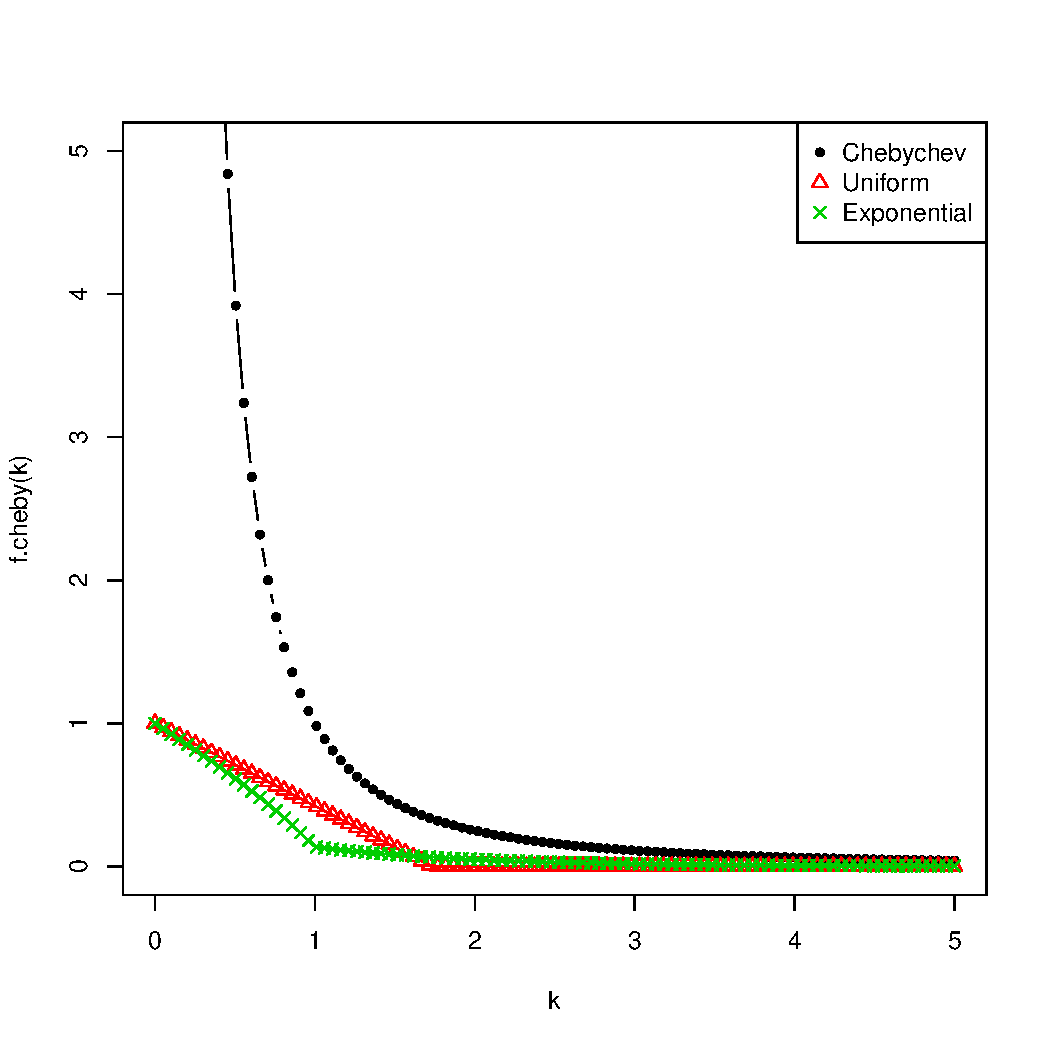
\includegraphics[width=4in]{chebychev.pdf}
    \end{center}

    And clearly we can see that from the plot, the bound is very conservative. 
\end{document}
